\section{概率质量与密度}
\label{sec:rvd-mass-density}

分布函数对所有随机变量都适用，但用它算概率并不总是最直接。抽检的次品数，一张三格的表就说完了；等待时间的分布函数是累计量，问“等待在$1.5$分钟附近有多集中”时，还得从它的变化率读出来。本节为两类常见情形各给一种更直接的表示：取值可以一一列出时，记录每个取值的概率；取值连续铺开时，记录单位长度上的概率。

\paragraph{概率质量函数}
骰子点数、次品数、首次成功前的试验次数，都只取有限或可数个值。对这类变量，最自然的描述是逐个列出取值和概率，就像上一节证明定理~\ref{thm:rvd-cdf-properties}时所用的表。

\begin{definition}[概率质量函数]
\label{def:rvd-pmf}
若存在有限或可数的集合$\{x_1,x_2,\dots\}$，使$X$只在其中取值，即$\sum_i\mathbb{P}(X=x_i)=1$，就称$X$为\term{离散随机变量}（discrete random variable）。函数
\begin{equation}
  p_X(x)=\mathbb{P}(X=x),\qquad x\in\mathbb{R}
  \label{eq:rvd-pmf}
\end{equation}
称为$X$的\term{概率质量函数}（probability mass function）。集合$\{x:p_X(x)>0\}$称为它的\term{支撑}（support）。
\end{definition}

质量函数满足两条：$p_X(x)\geq0$，且在支撑上的总和为$1$。按上一节对可数取值的约定，任何集合的概率都是其中各点质量之和：
\begin{equation}
  \mathbb{P}(X\in B)=\sum_{x_i\in B}p_X(x_i).
  \label{eq:rvd-pmf-sum}
\end{equation}
反过来，任给有限或可数个点和一组非负、总和为$1$的数，都能这样规定一个离散分布。离散分布的计算因此就是求和。

质量函数与分布函数互相确定。由式~\eqref{eq:rvd-pmf-sum}取$B=(-\infty,x]$，得到
\begin{equation}
  F_X(x)=\sum_{x_i\leq x}p_X(x_i);
  \label{eq:rvd-pmf-to-cdf}
\end{equation}
反方向，由式~\eqref{eq:rvd-jump}，$p_X(x)=F_X(x)-F_X(x^{-})$，即分布函数在$x$处的跳跃高度。图~\ref{fig:rvd-inspection-cdf}的两幅子图正是同一分布的两种表示。

\paragraph{可数个取值：首次掷出六点}
反复掷一枚公平骰子，记第一次出现六点时已掷的次数为$N$。事件$\{N=k\}$是“前$k-1$次都不是六点、第$k$次是六点”。各次投掷相互独立，由第~\ref{chap:classical-probability}章的乘法规则，
\begin{equation}
  p_N(k)=\Bigl(\frac56\Bigr)^{k-1}\frac16,\qquad k=1,2,3,\dots
  \label{eq:rvd-first-six}
\end{equation}
$N$可以取任意正整数，支撑是可数无限集。

先核对总质量。这是首项$1/6$、公比$5/6$的几何级数，
\[
  \sum_{k=1}^{\infty}\Bigl(\frac56\Bigr)^{k-1}\frac16=\frac16\cdot\frac{1}{1-5/6}=1 .
\]
再由式~\eqref{eq:rvd-pmf-to-cdf}求分布函数。对正整数$k$，前$k$项的部分和是
\[
  F_N(k)=\frac16\cdot\frac{1-(5/6)^{k}}{1-5/6}=1-\Bigl(\frac56\Bigr)^{k}.
\]
它也可以直接看出：$\{N>k\}$就是前$k$次都不是六点，概率为$(5/6)^{k}$。

图~\ref{fig:rvd-first-six}画出了质量函数和分布函数。分布函数在每个正整数处跳跃，跳跃无穷多次，却始终没有到达$1$；它与$1$的距离是尚未累计的尾部质量。例如掷了$10$次仍未出现六点的概率是$(5/6)^{10}\approx0.1615$，这正是定理~\ref{thm:rvd-cdf-properties}证明中“级数尾部可以任意小”的具体样子。

\begin{BookInlineFigure}
  \centering
  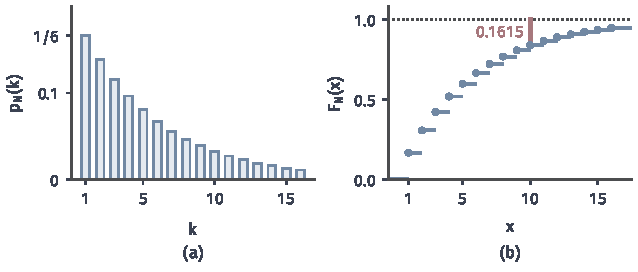
\includegraphics[width=108mm]{figures/07-probability/01-elementary-probability/matplotlib/rvd-first-six/figure.pdf}
  \caption{首次掷出六点所需次数$N$。(a)质量函数$p_N(k)=(5/6)^{k-1}/6$，只画出$k\leq16$；(b)分布函数$F_N$，在每个正整数处跳跃，点线是高度$1$。红线是$x=10$处尚未累计的质量$(5/6)^{10}\approx0.1615$。}
  \label{fig:rvd-first-six}
\end{BookInlineFigure}

\paragraph{核对一张概率表}
给出一张表时，要检查非负、总和为$1$，并说明支撑。设$X$取正整数，$p_X(k)=c/(k(k+1))$，常数$c$待定。把每一项拆成两个分数之差，部分和中间各项依次抵消：
\[
  \sum_{k=1}^{n}\frac{1}{k(k+1)}=\sum_{k=1}^{n}\Bigl(\frac1k-\frac1{k+1}\Bigr)=1-\frac1{n+1}.
\]
令$n\to\infty$，级数和为$1$，所以$c=1$。用同样的抵消，$\mathbb{P}(X\geq5)=1/5$，$F_X(k)=k/(k+1)$。这张表下一节还会用到：它的尾部衰减得很慢。

\paragraph{密度：单位长度上的概率}
等待时间的分布函数处处连续。对任意$t$和$h>0$，$\{T=t\}\subseteq\{t-h<T\leq t\}$，所以$\mathbb{P}(T=t)\leq F_T(t)-F_T(t-h)$，令$h\to0$即得$\mathbb{P}(T=t)=0$。每个单点的概率都是$0$，质量函数恒为零，提供不了任何信息。概率并没有消失，只是不再集中在一个个点上，而是像一根粗细不均的细棒上的质量那样沿实轴连续铺开。描述细棒，我们用线密度，即单位长度上的质量；某一段的质量是线密度在这一段上的积分。

先看一个能直接算出“单位长度上的概率”的例子。在半径为$1$的圆盘内随机取一点，规定点落在任一区域的概率等于该区域面积与圆盘面积$\pi$之比。记点到圆心的距离为$R$。$\{R\leq r\}$是半径$r$的小圆盘（图~\ref{fig:rvd-disk-radius}(a)），所以
\[
  F_R(r)=\frac{\pi r^{2}}{\pi}=r^{2},\qquad 0\leq r\leq1 .
\]
$r<0$时$F_R(r)=0$，$r>1$时$F_R(r)=1$。

\begin{BookInlineFigure}
  \centering
  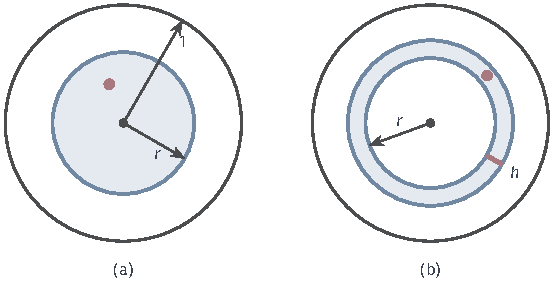
\includegraphics[width=94mm]{figures/07-probability/01-elementary-probability/tikz/rvd-disk-radius/figure.pdf}
  \caption{单位圆盘内随机取点（红点），$R$是它到圆心的距离。(a)事件$\{R\leq r\}$是浅蓝的小圆盘，概率为面积比$r^{2}$；(b)事件$\{r<R\leq r+h\}$是宽$h$的圆环，面积$\pi(2rh+h^{2})$，概率约为$2rh$。圆环越靠外越长，所以同样宽度的圆环外侧概率更大。}
  \label{fig:rvd-disk-radius}
\end{BookInlineFigure}

现在取一个宽$h$的圆环$\{r<R\leq r+h\}$（图~\ref{fig:rvd-disk-radius}(b)）。由式~\eqref{eq:rvd-interval}，
\[
  \mathbb{P}(r<R\leq r+h)=(r+h)^{2}-r^{2}=2rh+h^{2}.
\]
除以宽度$h$，得到这一段上平均每单位长度的概率：
\[
  \frac{\mathbb{P}(r<R\leq r+h)}{h}=2r+h .
\]
令$h\to0$，极限是$2r$。这就是$R$在$r$处的“单位长度上的概率”。

图~\ref{fig:rvd-density-histogram}把这个比值画成柱：每根柱的面积等于对应区间的概率，柱高是概率除以宽度。宽度从$0.25$缩小到$0.05$，柱顶越来越贴近直线$2r$。点在圆盘内是“均匀”取的，$R$却不均匀：离圆心越远，同样宽度的圆环越长，分到的概率越多。

\begin{BookInlineFigure}
  \centering
  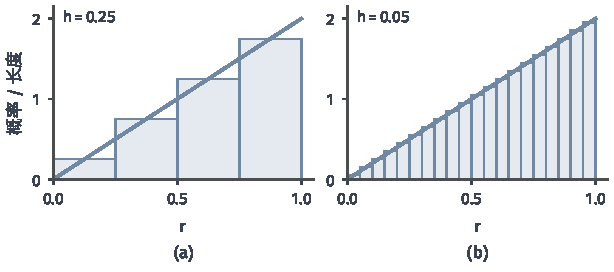
\includegraphics[width=104mm]{figures/07-probability/01-elementary-probability/matplotlib/rvd-density-histogram/figure.pdf}
  \caption{圆盘半径$R$的单位长度概率。浅蓝柱的宽度为$h$，高度为$\mathbb{P}(r<R\leq r+h)/h=2r+h$，面积就是该段的概率；蓝线是极限$2r$。(a)$h=0.25$；(b)$h=0.05$，柱顶与直线的差距缩小为$h$。}
  \label{fig:rvd-density-histogram}
\end{BookInlineFigure}

把这种描述作为定义：不再从分布函数出发求变化率，而是直接用一个函数的积分规定区间概率。

\begin{definition}[概率密度函数]
\label{def:rvd-density}
若存在非负函数$f_X$，使$\int_{-\infty}^{\infty}f_X(x)\,\mathrm{d}x=1$，并且对一切$a<b$都有
\begin{equation}
  \mathbb{P}(a<X\leq b)=\int_{a}^{b}f_X(x)\,\mathrm{d}x,
  \label{eq:rvd-density}
\end{equation}
就称$X$有\term{概率密度函数}（probability density function）$f_X$，简称密度。其中$a$可以取$-\infty$，$b$可以取$+\infty$，积分可以是反常积分。
\end{definition}

这里的积分是卷一意义下的黎曼积分，在无穷区间或被积函数无界时按反常积分理解，可参考\BookChapterRef{chap:univariate-integration}{卷一第7章“一元函数的积分”}。密度为正的范围称为它的支撑，例如$R$的支撑是$[0,1]$，等待时间的支撑是$[0,\infty)$。取$a=-\infty$，定义直接给出分布函数是密度的累计：
\begin{equation}
  F_X(x)=\int_{-\infty}^{x}f_X(t)\,\mathrm{d}t .
  \label{eq:rvd-cdf-from-density}
\end{equation}

\paragraph{密度模型的分布函数}
上一节对离散变量证明了分布函数的性质，现在对有密度的变量核验同样的性质，并看清单点概率为什么都是零。

\begin{theorem}[有密度时的分布函数]
\label{thm:rvd-density-cdf}
设$X$有密度$f_X$。则$F_X$单调不减、处处连续，$\lim_{x\to-\infty}F_X(x)=0$，$\lim_{x\to+\infty}F_X(x)=1$，并且对每个$x$都有$\mathbb{P}(X=x)=0$。若$f_X$在$x_0$处连续，则$F_X$在$x_0$处可导，且
\begin{equation}
  F_X'(x_0)=f_X(x_0).
  \label{eq:rvd-density-derivative}
\end{equation}
\end{theorem}

\begin{proof}
单调性来自被积函数非负：$x<y$时$F_X(y)-F_X(x)=\int_x^yf_X\geq0$。两端极限是反常积分$\int_{-\infty}^{\infty}f_X=1$收敛的定义：上限趋于$-\infty$时积分趋于$0$，趋于$+\infty$时积分趋于$1$。

连续性要证明$h\to0$时$\int_x^{x+h}f_X\to0$（$h<0$时理解为$-\int_{x+h}^{x}f_X$）。若$f_X$在$x$附近有界，设$\lvert f_X\rvert\leq K$，则这个积分的绝对值不超过$K\lvert h\rvert$，趋于$0$。若$f_X$在$x$附近无界，$x$是反常积分的瑕点，而反常积分收敛的定义正是积分上限（或下限）趋于瑕点时积分有极限，这个极限就是$F_X(x)$，所以积分同样趋于$0$。

单点概率：对$h>0$，$\{X=x\}\subseteq\{x-h<X\leq x\}$，于是
\[
  0\leq\mathbb{P}(X=x)\leq F_X(x)-F_X(x-h).
\]
由连续性，右边随$h\to0$趋于$0$，所以$\mathbb{P}(X=x)=0$。最后，$f_X$在$x_0$处连续时，式~\eqref{eq:rvd-density-derivative}是微积分基本定理对积分上限函数的结论。
\end{proof}

于是有密度的变量取任何一个具体值的概率都是$0$，而它每次总会取到某个值。这并不矛盾：实轴上有不可数多个点，概率是在区间上累计起来的，不是逐点相加起来的。“概率为零”与“不可能”在这里分开了：$\{T=1\}$是可能发生的事件，概率却为零。实际计算中的直接后果是端点开闭不再重要：
\[
  \mathbb{P}(a<X\leq b)=\mathbb{P}(a\leq X\leq b)=\mathbb{P}(a<X<b)=\int_a^bf_X(x)\,\mathrm{d}x .
\]

\paragraph{等待时间的密度}
式~\eqref{eq:rvd-waiting-cdf}的分布函数在$t\neq0$处可导，导数在$t<0$时为$0$，在$t>0$时为$\mathrm{e}^{-t}$。下面会说明，这样的分布函数由导数给出密度：
\[
  f_T(t)=\begin{cases}0,&t<0,\\\mathrm{e}^{-t},&t\geq0.\end{cases}
\]
图~\ref{fig:rvd-waiting-density-cdf}用两种方式表示同一个概率$\mathbb{P}(1<T\leq2)\approx0.2325$：在密度图中它是曲线下的面积，在分布函数图中它是两个函数值的高度差。密度越大的地方，分布函数上升越快。

\begin{BookInlineFigure}
  \centering
  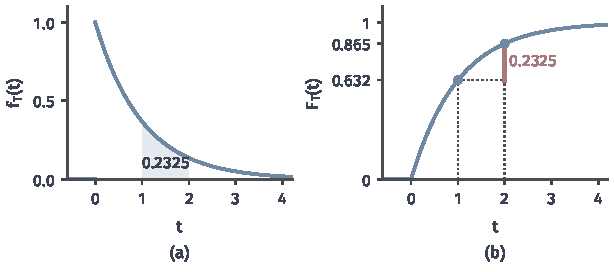
\includegraphics[width=104mm]{figures/07-probability/01-elementary-probability/matplotlib/rvd-waiting-density-cdf/figure.pdf}
  \caption{等待时间$T$的密度与分布函数。(a)密度$f_T(t)=\mathrm{e}^{-t}$（$t\geq0$），浅蓝面积是$\mathbb{P}(1<T\leq2)=\mathrm{e}^{-1}-\mathrm{e}^{-2}\approx0.2325$；(b)分布函数$F_T(t)=1-\mathrm{e}^{-t}$，同一概率是$t=2$与$t=1$处函数值之差（红线）。}
  \label{fig:rvd-waiting-density-cdf}
\end{BookInlineFigure}

\paragraph{由分布函数求密度}
定理~\ref{thm:rvd-density-cdf}说密度是分布函数的导数。反过来，什么时候能对分布函数求导得到密度？最常用的是下面这个充分条件。

\begin{theorem}[由分布函数求密度]
\label{thm:rvd-cdf-to-density}
设$F_X$处处连续，并且除有限个点$c_1<\dots<c_m$外连续可导，导数$F_X'$在每个开区间$(c_{k},c_{k+1})$上反常可积。令$f(x)=F_X'(x)$（在$c_k$处任意取非负值），则$f$是$X$的密度。
\end{theorem}

\begin{proof}
分布函数单调不减，所以导数$F_X'\geq0$，$f$非负。取$a<b$，在$a,b$之间插入落在其中的那些$c_k$，把$[a,b]$分成若干段。在每一段的内部，$F_X$连续可导，由Newton--Leibniz公式，$F_X$在段内两点之间的增量等于导数的积分；让两点趋于段端，$F_X$的连续性保证增量趋于整段的增量，积分按反常积分收敛到整段的积分。各段相加，得到
\[
  F_X(b)-F_X(a)=\int_a^bf(x)\,\mathrm{d}x .
\]
这就是式~\eqref{eq:rvd-density}。令$a\to-\infty$、$b\to+\infty$，由分布函数的两端极限得到$\int_{-\infty}^{\infty}f=1$。有限个点处的取值不影响积分。
\end{proof}

圆盘半径$R$满足条件：$F_R$连续，除$r=0,1$外可导，于是$f_R(r)=2r$（$0<r<1$），其余处为$0$，正是前面由圆环得到的极限。用它验算：
\[
  \mathbb{P}(0.5<R\leq1)=\int_{0.5}^{1}2r\,\mathrm{d}r=1-0.25=0.75 .
\]
从分布函数直接算是$F_R(1)-F_R(0.5)=0.75$，两者一致。条件中的“连续”不能去掉：抽检次品数的分布函数除三个点外导数都是零，按导数得到的“密度”积分为$0$，丢掉了全部质量。第~\ref{sec:rvd-representation-limits}节还会看到，即使分布函数连续，也可能求不出密度。

\paragraph{密度值不是概率}
密度的单位是“概率每单位长度”，它的值本身不是任何事件的概率。若$f_X$在$x$处连续，由积分中值定理，存在$\xi_h\in[x,x+h]$使
\[
  \mathbb{P}(x<X\leq x+h)=f_X(\xi_h)\,h\approx f_X(x)\,h .
\]
所以只有乘上一小段长度，密度才变成概率。密度的值可以大于$1$，甚至可以无界，只要曲线下的总面积是$1$。

图~\ref{fig:rvd-density-values}给出三个例子。(a)在$(0,1/2)$上$f(x)=2$，其余处为$0$，总面积$2\times\frac12=1$，而
\[
  \mathbb{P}(0.1<X\leq0.3)=2\times0.2=0.4 .
\]
(b)在$(0,1)$上$f(x)=6x(1-x)$，最大值$f(1/2)=1.5$，下面还会用它演示怎样核对密度。(c)在$(0,1]$上$f(x)=1/(2\sqrt{x})$，在$0$附近无界，但反常积分收敛，分布函数是$F(x)=\sqrt{x}$（$0\leq x\leq1$），于是
\[
  \mathbb{P}(X\leq\tfrac14)=\sqrt{1/4}=\tfrac12 .
\]

\begin{BookInlineFigure}
  \centering
  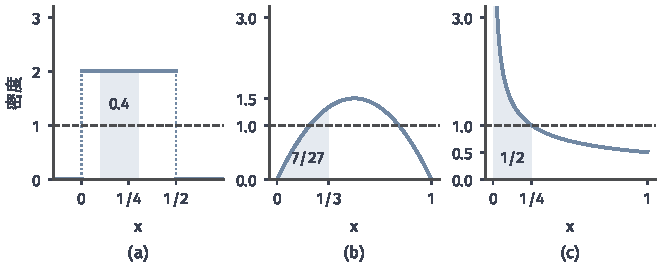
\includegraphics[width=112mm]{figures/07-probability/01-elementary-probability/matplotlib/rvd-density-values/figure.pdf}
  \caption{密度的高度不是概率。虚线是高度$1$，浅蓝面积是所标的概率。(a)$(0,1/2)$上的常数密度$2$，$\mathbb{P}(0.1<X\leq0.3)=0.4$；(b)$6x(1-x)$，最大值$1.5$，$\mathbb{P}(X\leq1/3)=7/27$；(c)$1/(2\sqrt{x})$在$0$附近无界，$\mathbb{P}(X\leq1/4)=1/2$。}
  \label{fig:rvd-density-values}
\end{BookInlineFigure}

密度值还依赖于单位。等待时间以分钟计时密度在$0$处等于$1$；改以小时计，$H=T/60$，于是对$s\geq0$，
\[
  \mathbb{P}(H\leq s)=\mathbb{P}(T\leq60s)=1-\mathrm{e}^{-60s}.
\]
求导得
\[
  f_H(s)=60\,\mathrm{e}^{-60s},\qquad s\geq0,
\]
在$0$处等于$60$。同一事件的概率不随单位改变，单位长度上的概率却要按长度单位换算。

\paragraph{核对一个函数是不是密度}
给出候选密度时，要核对三件事：在支撑上非负，总积分为$1$，支撑写清楚。设$f(x)=c\,x(1-x)$（$0<x<1$），其余处为$0$。在$(0,1)$上$x(1-x)>0$，非负性只要求$c>0$。归一化要求
\[
  c\int_0^1x(1-x)\,\mathrm{d}x=c\Bigl(\frac12-\frac13\Bigr)=\frac c6=1,
\]
所以$c=6$，这就是图~\ref{fig:rvd-density-values}(b)。它的分布函数是
\[
  F(x)=\int_0^x6t(1-t)\,\mathrm{d}t=3x^{2}-2x^{3},\qquad 0\leq x\leq1,
\]
所以$\mathbb{P}(X\leq1/3)=3/9-2/27=7/27\approx0.259$。

支撑不能随意扩大。若把同一公式用在$(0,2)$上，$1<x<2$时$x(1-x)<0$，无论$c$取什么正数都违反非负性；把公式写成“$f(x)=6x(1-x)$”而不写支撑，读者就无从判断它在区间外是什么。

\paragraph{从细格上的质量到密度}
质量与密度的关系可以通过把格子越分越细看出来。设$X_n$以概率$1/n$取$1/n,2/n,\dots,n/n$中的每一个值，相邻取值相距$1/n$。每一点的质量$1/n$随$n$增大趋于$0$，但质量除以格宽始终是
\[
  \frac{1/n}{1/n}=1 .
\]
分布函数是$F_{X_n}(x)=\lfloor nx\rfloor/n$（$0\leq x\leq1$），它与$x$的差不超过$1/n$。

当$n\to\infty$时，阶梯越来越密、台阶越来越矮，分布函数逼近$F(x)=x$，这正是$(0,1)$上常数密度$1$的分布函数。质量函数的值趋于零，提供不了极限的信息；分布函数和“质量除以格宽”却都有好的极限。所以比较离散与连续的模型时，要拿分布函数比，或者拿“质量/格宽”与密度比，不能拿单点质量与密度值比。分布怎样在这种意义下逼近，在第~\ref{chap:random-variable-convergence}章系统研究。

\paragraph{密度只在积分意义下确定}
改变$f_X$在有限个点处的值，所有区间上的积分都不变，因而规定的是同一个分布。所以“$X$的密度”实际上指一族只在有限个点处不同的函数，我们总选其中最方便的一个，例如在支撑的端点处取什么值都可以。与此不同，质量函数在每一点的值都有意义，改动任何一点都会改变分布。这也说明密度在单点上的值不能单独解释，只有它在小区间上的平均才对应概率。

表~\ref{tab:rvd-mass-vs-density}对比了两种表示。

\begin{BookInlineTable}
  \centering
  \begin{tabular}{lll}
    \toprule
    & 质量函数$p_X$ & 密度$f_X$\\
    \midrule
    区间概率 & 对取值求和 & 在区间上积分\\
    函数值 & 单点概率，不超过$1$ & 单位长度的概率，可大于$1$\\
    单点概率 & $p_X(x)$ & 恒为$0$\\
    分布函数 & 阶梯，跳跃高度为$p_X$ & 连续，导数为$f_X$\\
    端点开闭 & 可能改变结果 & 不影响结果\\
    改动一点的值 & 改变分布 & 不改变分布\\
    \bottomrule
  \end{tabular}
  \caption{概率质量函数与概率密度函数的对比。两者都要求非负、总量为$1$；区别在于质量集中在可数个点上，还是沿实轴连续铺开。}
  \label{tab:rvd-mass-vs-density}
\end{BookInlineTable}

习惯上把有密度的分布称为连续分布，把离散随机变量的分布称为离散分布。“连续分布”这个名字只说明分布函数连续；第~\ref{sec:rvd-representation-limits}节会看到，分布函数连续并不保证密度存在。
